\documentclass[12pt,letterpaper]{article}

% just for the example
\usepackage{lipsum}
% Set margins to 1.5in
\usepackage[margin=1.5in]{geometry}
\usepackage[toc,page]{appendix}

% for graphics
\usepackage{graphicx}
\graphicspath{{./figures/m1/}}

% for crimson text
\usepackage{crimson}
\usepackage[T1]{fontenc}
\usepackage{url}

% setup parameter indentation
\setlength{\parindent}{0pt}
\setlength{\parskip}{6pt}

% for 1.15 spacing between text
\renewcommand{\baselinestretch}{1.15}

% For defining spacing between headers
\usepackage{titlesec}
% Level 1
\titleformat{\section}
  {\normalfont\fontsize{18}{0}\bfseries}{\thesection}{1em}{}
% Level 2
\titleformat{\subsection}
  {\normalfont\fontsize{14}{0}\bfseries}{\thesection}{1em}{}
% Level 3
\titleformat{\subsubsection}
  {\normalfont\fontsize{12}{0}\bfseries}{\thesection}{1em}{}
% Level 4
\titleformat{\paragraph}
  {\normalfont\fontsize{12}{0}\bfseries\itshape}{\theparagraph}{1em}{}
% Level 5
\titleformat{\subparagraph}
  {\normalfont\fontsize{12}{0}\itshape}{\theparagraph}{1em}{}
% Level 6
\makeatletter
\newcounter{subsubparagraph}[subparagraph]
\renewcommand\thesubsubparagraph{%
  \thesubparagraph.\@arabic\c@subsubparagraph}
\newcommand\subsubparagraph{%
  \@startsection{subsubparagraph}    % counter
    {6}                              % level
    {\parindent}                     % indent
    {12pt} % beforeskip
    {6pt}                           % afterskip
    {\normalfont\fontsize{12}{0}}}
\newcommand\l@subsubparagraph{\@dottedtocline{6}{10em}{5em}}
\newcommand{\subsubparagraphmark}[1]{}
\makeatother
\titlespacing*{\section}{0pt}{12pt}{6pt}
\titlespacing*{\subsection}{0pt}{12pt}{6pt}
\titlespacing*{\subsubsection}{0pt}{12pt}{6pt}
\titlespacing*{\paragraph}{0pt}{12pt}{6pt}
\titlespacing*{\subparagraph}{0pt}{12pt}{6pt}
\titlespacing*{\subsubparagraph}{0pt}{12pt}{6pt}

% Set caption to correct size and location
\usepackage[tableposition=top, figureposition=bottom, font=footnotesize, labelfont=bf]{caption}

% set page number location
\usepackage{fancyhdr}
\fancyhf{} % clear all header and footers
\renewcommand{\headrulewidth}{0pt} % remove the header rule
\rhead{\thepage}
\pagestyle{fancy}

% Overwrite Title
\makeatletter
\renewcommand{\maketitle}{\bgroup
   \begin{center}
   \textbf{{\fontsize{18pt}{20}\selectfont \@title}}\\
   \vspace{10pt}
   {\fontsize{12pt}{0}\selectfont \@author} 
   \end{center}
}
\makeatother

% Used for Tables and Figures
\usepackage{float}

% For using lists
\usepackage{enumitem}

% For using APA Citation format
\usepackage{apacite}

% Custom Quote
\newenvironment{myquote}[1]%
  {\list{}{\leftmargin=#1\rightmargin=#1}\item[]}%
  {\endlist}
  
% Create Abstract 
\renewenvironment{abstract}
{\vspace*{-.5in}\fontsize{12pt}{12}\begin{myquote}{.5in}
\noindent \par{\bfseries \abstractname.}}
{\medskip\noindent
\end{myquote}
}

\begin{document}

% Set Title, Author, and email
\title{Assignment M2}
\author{Snejana Shegheva \\ sshegheva3@gatech.edu}

\maketitle
\thispagestyle{fancy}

\begin{abstract}
Mapping data from one form to another for its ease-of-use is at the core of the \textit{Extract, Transform and Load} process \cite{wiki:etl}. There exist many tools that can accomplish the task of creating and maintaining a data warehouse. However, sometimes it is advantageous to have a custom solution that allows a user to interact with the data directly during some or all of the ETL phases. In this project, we analyze an internal interface of a \textit{transform} task that prepares the data for use in a personalized recommendation system powered by Artificial Intelligence engines. Our main goal is to assess all the weak areas of the existing interface in order to provide recommendations for alternative models that simplify the user interaction without assuming any pre-existing knowledge of the tool.
\end{abstract}

\subsection*{Needfinding Plan 1 - Participant Observation}
In the Participant Observation approach we experience the task ourselves and record both, the steps performed and their outcomes in order to analyze effectiveness and usability of the interface for the given task. 

To get started with a transformation task, I first need to get input data. For this project, I chose to retrieve data from the website \textit{http://arxiv.org} that provides an open access to papers in Physics, Mathematics, Computer Science, and other fields. After loading the data into the system and extracting 30 fields, such as \textit{authors}, \textit{title}, \textit{summary}, \textit{published}, etc., I was presented with a view that allows seeing each property's metadata - \textit{id}, \textit{name}, \textit{data type}, and an option to \textit{Edit} the property. Pressing the \textit{Edit} button enters the interface portion that deals with transformation task for a chosen property.    

\textbf{Goal}: From a data property, \textit{published}, that has a format \textit{dd-mm-yy}, I wish to extract the \textit{year} portion only so I can possibly perform other statistics with this field. 

\textbf{Task}: Find the original property \textit{published}, transform it into a new property that keeps only the last two digits, and store the result in a \textbf{new} property \textit{year}.

After briefly looking at the list of available transformation functions, the closest candidate I found was \textit{RegexTransformer}, an internal wrapper over the regular expression language \cite{wiki:regex}. This prompted a new \textbf{subtask}: generate a correct expression that finds the last two digits in a string. Trial, error and Google eventually led me to an expression "{\textbackslash{d}\{2\}\$}" that provided output I was expecting.

\textbf{Observations}:

1) The list of available transformations is very large (over 30), and I had to go through at least five of them until I stumbled on \textit{RegexTransform}. There is no classification of the transformation functions available that can help narrow down the search.

2) I was hoping to find a transformation that \textit{knows} how to deal with dates directly that can support multiple date formats. Although, I did not find a an exact operation, the system provided me with a generic type of transformation that I could mold to suit my task.

3) The largest interface limitation that I have noticed is \textbf{constraining} user to select a single source property for which to perform a transformation. I can imagine a case where I would want to subtract two dates, for example \textit{submitted date} and \textit{published date}, to gain some insignts on the publication process.

In this needfinding plan, it was very hard to avoid the \textit{Confirmation} bias, since, as a Data Scientist dealing with data manipulations on a daily basis, I have a strong opinion on what an interface designed for transformations should support. To control for that, I complimented this needfinding approach with \textit{Interviews}, so I can gather perspectives from users of different roles. 

\subsection*{Needfinding Plan 2 - Interviews}
With the Participant plan, we have addressed questions such as \textit{What are the users' goals} and \textit{What are their tasks}. To understand \textit{Who are the users} and \textit{What is the context of the task}, I interviewed four of my colleagues who also interact with the interface being analyzed. I specifically selected them based on their roles as together they represent a large variety of user types. 

\textbf{Who} are the users and \textbf{What} are their \textbf{contexts}:

1) Product Manager / Client Lead - Deals with the interface on the daily basis from the business perspective: load customer's data during early phases to understand their problem space, and how the overall product needs customer's needs.

2) Chief Technology Officer (CTO) - Similarly to the Product Manager, evaluates the customer's needs with early prototypes that involve significant data manipulations and enrichment.

3) UX Designer - Does not work directly with the transformation task since they do not deal with data, however, is closely aware of the interface being discussed.   

4) Software Architect - Does not need to work with transformations on daily basis, however, need to considers the overall system's capabilities.

The interview questions covered a broad aspect of the interface, focusing on three areas - Data Presentation, Data Transformation and Feedback. The full list of questions is available in the \textit{Appendix A}. The raw answers, based on the verbal interviews, are available in the \textit{Appendix B}. 

\textbf{Takeaways}:

1) The workflow of the interface is not very intuitive, and it lacks \textit{wizard-like} features to walk the user through the setup.

2) The interface does not follow a standard design (button positions) that leads to a confusion on the sequence of steps. For example, the interface currently has a great way to provide an immediate feedback by letting the user \textit{try} the transformation; however, because the designated location of this functionality is \textit{below} the \textit{Save} button, it is not clear if selected transformation is \textit{Applied} to the entire set.

3) Generalization vs. Flexibility. Re-designing an interface must consider the trade-offs between how much flexibility it has (addressing the needs for very specialized audiences) and how many different users it can serve.

\textit{Recall} is an important bias in conducting interviews since studies have shown that people do not always remember their experiences accurately. To control for that, I selected some users with a significant experience with the tool (more than four years). For the new users, I conducted the interview \textit{right} after they went through the task.  

This approach for needfinding turned out to be surprisingly effective in collecting different perspectives on the same task. It forced me to re-think my original priority for features that need redesign, and to consider the additional load on the system especiallty in the case for only marginally improved user's experience.

\iffalse 
THIS IS COPIED FOR INSPIRATION
The main bias I expect to encounter with the interviewis recallbias. The user may remember things differently, or have difficulty remembering during the interview. To combat this, I will need to carefully analyze the data coming from the interview and compare it with the data from theother needfinding methods. Being aware and consciousof this bias should be sufficient for combating it. 
\fi

\subsection*{Needfinding Plan 1 - Hacks and Workarounds}
We have briefly described what the user's ultimate goal is, and how that can be broken down into sub-goals. In this section, we are going to further zoom into the user's actions for performing the task of data transformation. As our objective is to understand the weaknesses of the existing interface, as shown in Figure~\ref{fig::2}, we analyze the cases where the user breaks out of the provided interface and resorts to various hacks and workarounds to accomplish the task. A user in a Data Scientist role has a frequent need for manipulating the raw data that moves through the ETL pipeline. The main reasons why the user in that role currently changes their intended workflow and performs a subset of the actions outside of the given interface can be summarized by the following three categories: 

\begin{enumerate}
    \item \textbf{Limited functionality}. Before deciding on the transformation rules, a user needs to have a visibility on the data being transformed. In the current interface (see Figure~\ref{fig::3}), user selects the targeted data field, for example a \textit{published date}, and is given an \textit{edit} button. However, the interface does not provide enough information to make a fully informed action on the required transformation rule. Therefore, a workaround\#1:  
    \textit{Load the data in the external interface (command line, Jupyter notebooks, database queries) to explore descriptive statistics of the original field - the most frequent values,  the extreme values, the rate is missing fields, etc.}
    
    \begin{figure}[h]
    \centering
    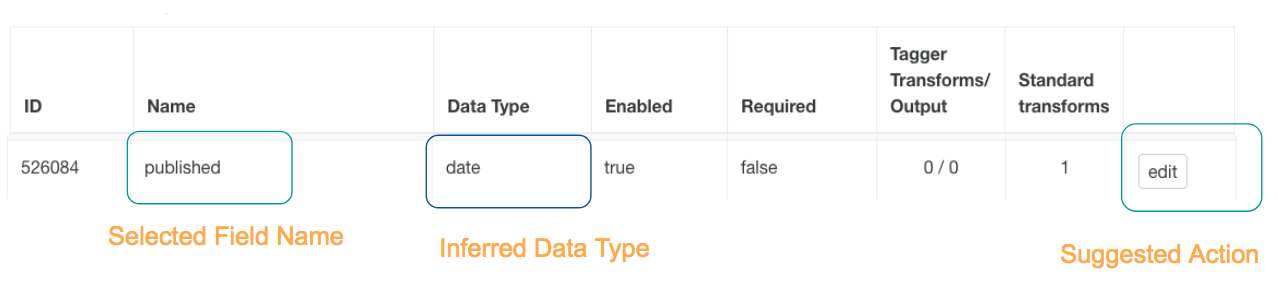
\includegraphics[width=4in, scale=.4]{DataVisibility.png}
    \caption{An example of the interface limitation to provide the user with knowledge of the present data form to enable an informed action.}
    \label{fig::3}
    \end{figure}
    
    
    \item \textbf{Poor Feature Organization}. After the user has decided on the transformation rule, the next step is to map their intentions to one of the of existing transformers. Figure~\ref{fig::4} shows that in the current interfaces the selection is given without consideration for priority or relevance of the transformation to the field being examined. Therefore, a workaround\#2:
    \textit{Browse through previously made transformations (if available) for examples and common use cases, ask colleagues for a bit of advice, or make educated guesses until the right transformer is found}
    
    \begin{figure}[h]
    \centering
    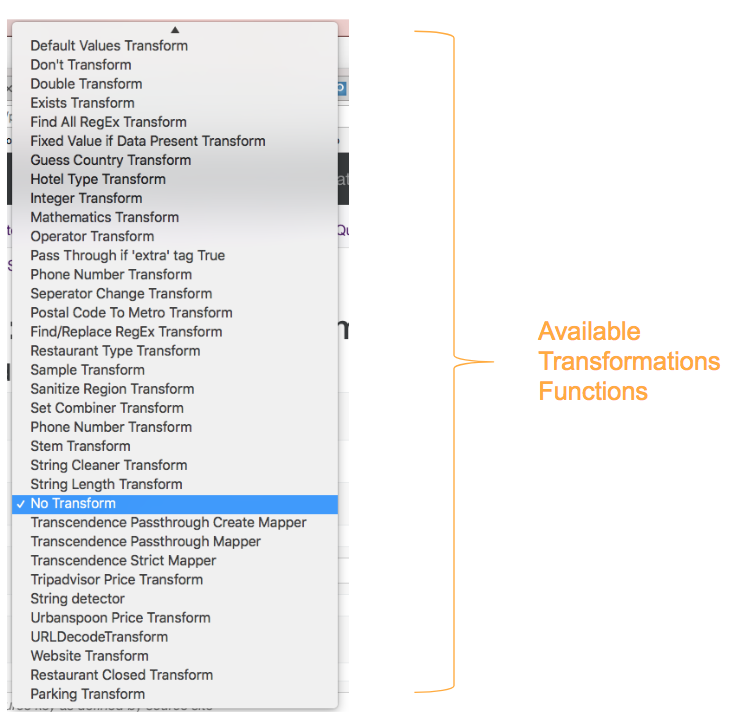
\includegraphics[width=4in, scale=.3]{Transformers.png}
    \caption{An example of the interface that displays ALL available transformation functions without priority or relevance consideration.}
    \label{fig::4}
    \end{figure}
    
    \item \textbf{Bugs in the existing functionality}. Unintended behavior in software happens all the time. The interface needs to provide accessible means to recover from a mistake by undoing an erroneous operation. A user should be comfortable exploring the interface without the fear of irreversibly corrupting the data. A good interface, therefore, should be able to guide the user from the failed state. As the current interface does not provide visibility on the original or the final data (after the applied transformation), there are no means to undo an action where transformation has the unintended effect. Workaround\#3: \textit{Modify the data via direct database access from, hopefully existing, backups.} 
    
\end{enumerate}

New type of bias: status quo:

\iffalse 

THIS IS COPIED FOR INSPIRATION: remove it!
In this needfinding method, there is little potential for bias. Possibly, we might en-counter status quo bias. Status quo bias occurs when there is an emotional preferencefor the current state of affairs. We might look at an alternate existing interface and feelthat if it is too different than what we are used to, that this would be a negative thing.To avoid this bias, we will go into the needfinding method with an open mind and theattitude that, for now, nothing is off the table.
\fi

The need-finding approach covered in this section connects the user's goals of altering a data feed to the sub-tasks of viewing the existing data, planning the transformation, and confirming the outcome. The approach of need-finding via analysis of hacks and workarounds is susceptible to \textit{observational selection bias} as we tend to notice workarounds when they impact us directly. To avoid this bias, we pair up this approach with another method that seeks to understand the pain points of a larger group of users, preferably with diverse roles.


To better understand the user's struggles with the interface, it is useful to analyze the frequencies of two kinds of errors, such as \textit{slips} and \textit{mistakes}. A mental model is a process that explains how a user is thinking about the task regarding actions and outcomes \cite{wiki:mental_model}. When a mental model matches the logic implemented by an algorithm, the user has a correct understanding of the system's functionality. In this case, the user's error can be classified as a slip vs. a mistake where the user has a wrong mental model. The approach for need-finding that focuses on error analysis broadens the spectrum of users in terms of their expertise in the given task. A novice in the field can be guided through the process of transformation by automatically matching the compatible functions to the field subjected to alterations. 

Figure~\ref{fig::5} exemplifies a hypothetical scenario where the user does not have a correct representation of the state and appropriate actions. In this example, the user attempts to transform a field that captures a person's name (\textit{author}) by applying a function that is designed to manipulate \textit{dates}. This is an incompatible operation that should not be allowed by the interface. The analysis of errors for such type outlines a \textit{need} for system's intelligence to understand the input data types and the \textit{schemata} of the available transform to reduce the space of possible matches. An improvement like can decrease the chances for user to apply incorrect action for the task at hand.   

\begin{figure}[h]
\centering
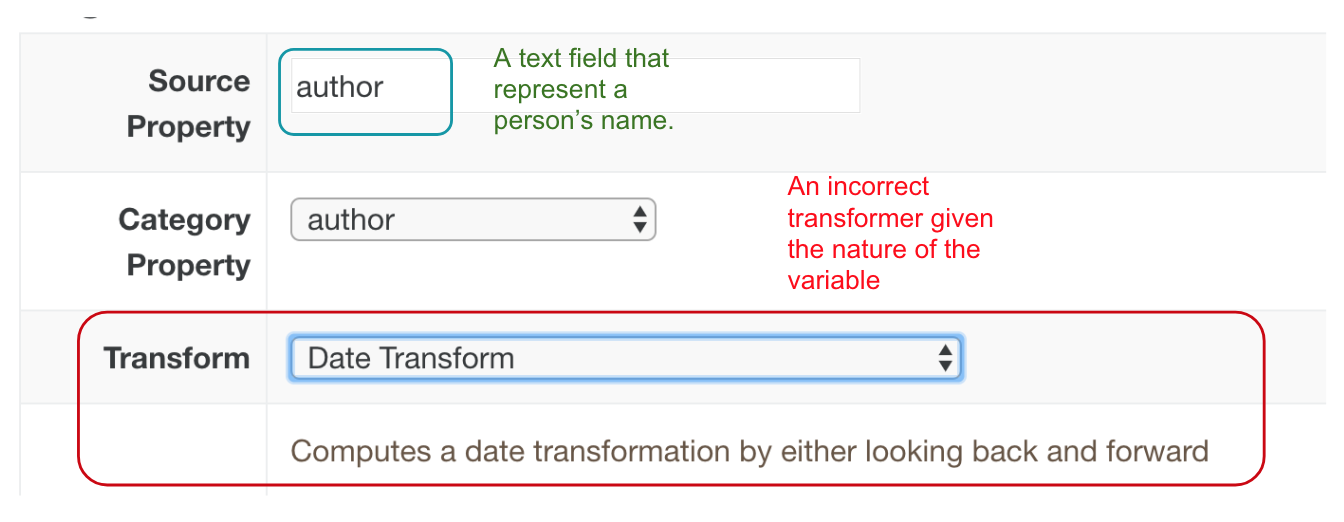
\includegraphics[width=4in, scale=.3]{mistake.png}
\caption{An example of the incorrect user action where their mental model of the underlying process is incorrect. A textual field, such as person's name cannot be computed as a date transformation.}
\label{fig::5}
\end{figure}

When a user has a correct mental model, but still makes an error due to a rushed behavior, there is an opportunity to improve the interface to reduce the chance of \textit{slippage} by altering the nature of interactions. Figure~\ref{fig::6} shows an interface that expects the user to submit a list of characters for String Cleaning. This form of interaction allows easy creation of a typo that can be avoided by modifying the underlying interaction. A change like an abstraction of special characters into a class of invalid characters for a \textit{name} field can improve users' efficiency in performing a transformation task.

\begin{figure}[h]
\centering
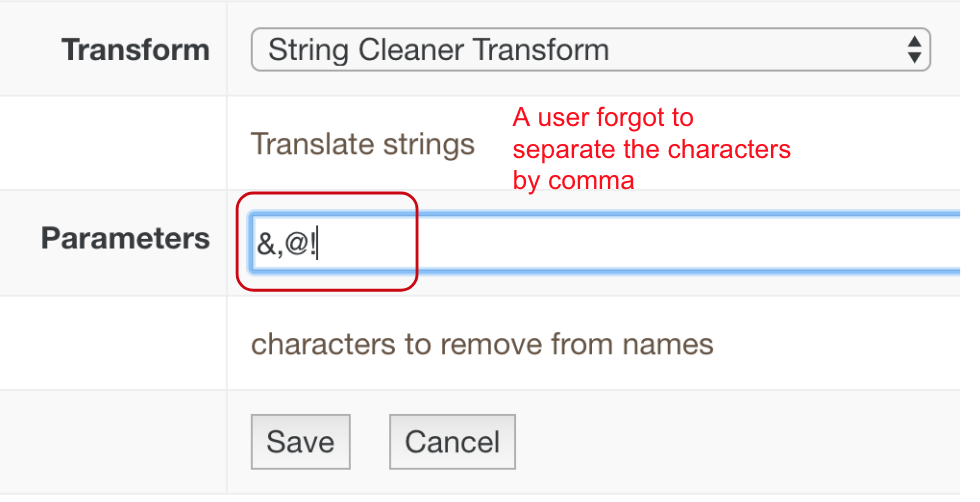
\includegraphics[width=4in, scale=.3]{slip.png}
\caption{An example of the incorrect user action where their mental model of the underlying process is correct, but user can still easily make a mistake by making a typo.}
\label{fig::6}
\end{figure}

Similarly to the approach of Hacks and Workaround, the Error analysis approach is susceptible to the \textit{observational selection} bias. In both methods, the effect of the bias can be reduced by quantitatively measuring the impact those errors have on the productivity of the end users. Metrics such as time spent troubleshooting the errors, likelihood of data corruption/loss, resources requires to re-design the specific components of the interface, etc. can help prioritize one types of errors over others.  






\bibliographystyle{apacite} 
\bibliography{bibtemp}

\appendix

\section{Interview Questions}

\subsubsection*{Section 1 - Data Presentation}
When deciding to transform a property, what is the value for you in being able to see the sample of existing data for the given property? If you do not see a value on that, please explain why.  If you see a value, please provide a recommendation on what constitutes a good sample, for example, you want to see the most recent values, the most frequent values, the most extreme values, etc. If you choose to say "yes" to the value, then please justify your needs. Here, you can describe your role, and why is this important to you.  

\subsubsection*{Section 2 - Data Transformation}
How frequently the data you loaded requires additional manipulation? What are your typical scenarios for transformations? When transforming a variable, do you need access to the other variables in a single record? What is one type of transformation that you need/want the most?  

\subsubsection*{Section 3 - Feedback/Recovery}
Do you feel that the current system's feedback is adequate? For example, recall scenarios where you wanted to transform a variable, but were struggling with the interface in terms of selecting needed information (selecting a transform type, configuring the transform, etc). What is your experience at the times where the transformation you applied had an unexpected effect? Did you have enough information to understand the issue and/or recover your data and re-iterate the process?

\section{\\Interview Raw Responses}

\subsection*{Role: Senior Product Manager, Client Lead}
\subsubsection*{Question 1 - Data Presentation} 

\begin{itemize}
    \item I end up going through this process for at least half of our customers
    \item Data presentation is helpful, but only crticial when a more complicated transformation is required (e.g. regex). Typically, I will look at the data PRIOR to this screen because I need to make the decision to do the transformation before I land here. 
    \item Once on this screen, it would be helpful to see the 'would be' output before it's changed.
    \item NOTE: this screen is currently just a config, not a processing screen. A more seamless flow would be very helpful!
\end{itemize}

\subsubsection*{Question 2 - Data Transformation}
\begin{itemize}
    \item I tend to think that an Excel/CSV/DB table format is the easiest way to look at this data (horizontally, one record per row). This is the way we load data into the system initially, too, so I'm already familiar with looking at data in this format. 
    \item Probably my most frequent transforms at this point are concatenatipne (combining two or more values) or trimming/parsing/stripping from fields (e.g. removing characters)
    \item I don't do bucket transforms here, probably because I find them too difficult/not intuitive
    \item The dropdown has MANY transforms I have never used... largely because I don't know what they do. 
    \item The parameters field is applied inconsistently and isn't clear. What is supposed to go there? How do we configure these params? Better documentation needed.
    \item On my wishlist - it would be great to configure transcendence/standardization at this point too. Transcendence and tagging both feel like transforms to me.
\end{itemize}

\subsubsection*{Question 3 - Feedback/Recovery}
\begin{itemize}
    \item I think the issue here is two-fold. 1. This is just a configuration screen... It doesn't actually kick off any processing, so you could set this and never see the outcome. 2. We don't have an easy way to see the processed data until it is moved to the platform (aka production). Exposing these in a staging area would be ideal.
    \item There are additional steps required to get the data wired all the way through to 'final output' (e.g. the partner property). 
    \item Correcting errors is especially hard with our data processing tool. I believe we update a transform and reprocess to the correct values, but I'm not sure if that catches everything or if old/bad data can remain (e.g. if you mistakenly use a transform that in one case yields a value for a source entity... if you correct it, so now that new source entity has no value, does the old value go away?
\end{itemize}

\subsection*{Role: Chief Technical Officer}
\subsubsection*{Question 1 - Data Presentation}

\begin{itemize}
    \item Not using mental energy to imagine how data looks like before the transformation is very important to me; This allows to focus on the interface. Plus, imagination could be exhausting :)
\end{itemize}

\subsubsection*{Question 2 - Data Transformation}
\begin{itemize}
    \item I am involved in rapid prototyping for a variety of clients. During this phase, the data we get is very unclean, therefore I have to perform a lot of transformations.
    \item Main areas of transformations: Dictionary Mappings, Combining fields, Cleaning Up.
\end{itemize}

\subsubsection*{Question 3 - Feedback/Recovery}
\begin{itemize}
    \item \textit{Try it} functionality we currently have is a great way to provide a feedback in the form of almost interactively reshaping the data
    \item An area where I stumble is around naming for the current transforms. Name is not always representative.
\end{itemize}

\subsection*{Role: Lead UX Designer}
\subsubsection*{Question 1 - Data Presentation}

\begin{itemize}
    \item It would be great to have a sneak peak into the data, however, one should be careful about not distracting the user from the task. Essentially, if the action of taking a look at the data underneath requires selecting multiple options, it does not improve user's experience overall. 
\end{itemize}

\subsubsection*{Question 2 - Data Transformation}
\begin{itemize}
    \item Although, I am not currently using this feature, I can imagine a need in a transformation that requires multiple variables.
\end{itemize}

\subsubsection*{Question 3 - Feedback/Recovery}
\begin{itemize}
    \item The main advice in providing a good feedback to the user is being consistent with the standard interfaces (buttons especially). For example, the actions should be ordered as \textit{Cancel}, \textit{Apply}, and \textit{Save}. In our case, \textit{Try it} button is below \textit{Save} which might confuse the user.
\end{itemize}

\subsection*{Role: Software Architect}

Note: For this interview, I did not have a chance to record the answers immediately, so I paraphrased their main takeways
\subsubsection*{Question 1 - Data Presentation}

\begin{itemize}
    \item Although it is noble goal to show user teh sample of the data, what needs to be considered carefully is scalabillity of such requests. Would this additional feature, although nice, interfere with the overall task.  
\end{itemize}

\subsubsection*{Question 2 - Data Transformation}
\begin{itemize}
    \item Too many transformations can be generalized and combined into a single function. No need to be too granular in what each function can do.  
\end{itemize}

\subsubsection*{Question 3 - Feedback/Recovery}
\begin{itemize}
    \item The users currently may suffer from system's frugal messaging when something goes wrong, and its overly verbosity for the typical workflow.
\end{itemize}

\end{document}
